%! Author = Philipp Emmenegger
%! Date = 09/07/2021

\section{React}
Library, kein Framework.
Um UIs zu bauen.
View in MVC.
Minimales Featureset.

\subsubsection{Prinzipien}
\begin{itemize}
    \item Komplexes Problem aufteilen in einfachere Komponenten
    \item Für eine bessere: Wiederverwendbarkeit, Erweiterbarkeit, Wartbarkeit, Testbarkeit, Aufgabenverteilung
\end{itemize}

\subsection{Entwicklung von UIs}
Beschreibung des UIs.
Event-Handling.
Aktualisieren der Views.

\subsection{Komponenten und Elemente}
\begin{itemize}
    \item Funktionen die HTML zurückgeben
    \item Beliebige Komposition von React-Elementen und DOM-Elementen
\end{itemize}
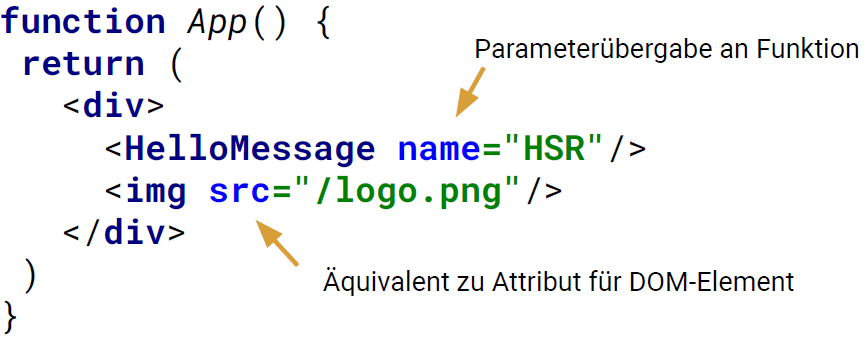
\includegraphics[width=0.6\linewidth]{img/react_component.png}

\subsection{JavaScript XML}
React verwendet JSX (blau), eine Erweiterung von JavaScript (gelb).
Überall wo JSX verwendet wird, muss $react$ importiert werden.\\
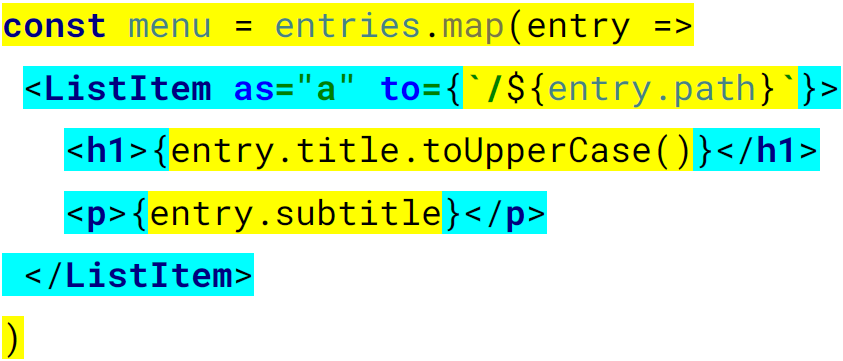
\includegraphics[width=0.6\linewidth]{img/react_jsx.png}\\
\textbf{Styles:} werden nicht als Strings sondern als Object angegeben.

\subsubsection{Props}
Komponenten erhalten alle Parameter/Properties als \textbf{props} Objekt.
$this.props$ bei Klassen.
Bei Funktionen als Parameter.
Immer \textbf{read-only}.

\subsubsection{Rendering und Mounting}
\begin{lstlisting}
ReactDOM.render(
    <App/>
    document.getElementById('root')
)
\end{lstlisting}

\subsection{React State}
Veränderbarer Zustand von Komponenten.
Ist immer privat.
Ändert der State, wird auch die Komponente aktualisiert.
\begin{lstlisting}
class Counter extends React.Component {
    state = { counter: 0 }
    // ...
}
\end{lstlisting}

\subsubsection{Event Handler}
\begin{lstlisting}
const increment = () => {
    this.setState({counter: this.state.counter + 1})
} // ...
<button onClick={this.increment}>
\end{lstlisting}

\subsection{Reconciliation}
\begin{enumerate}
    \item React Komponenten werden als virtueller DOM gerendert
    \item Wird der \textbf{state} geändert, erstellt React einen virtuellen DOM
    \item Alter und neuer DOM werden verglichen
    \item Erst dann werden geänderte DOM-Knoten im Browser erstellt
\end{enumerate}

\subsection{Komponenten Lifecycle}
\subsubsection{Mounting}
\textbf{1. constructor(props):} State initialisieren, sonst weglassen.
\textbf{2. getDerivedStateFromProps(props, state):} Von state abhängige Props initialisieren.
\textbf{3. render()}
\textbf{4. componentDidMount():} DOM ist aufgebaut. Guter Punkt um Async Daten zu laden. \textit{setState} führt zu re-rendering.

\subsubsection{Updating}
\textbf{1. getDerivedStateFromProps(props, state):} Von state abhängige Props aktualisieren.
\textbf{2. shouldComponentUpdate(nextProps, nextState):} render übersprungen bei false.
\textbf{3. render()}
\textbf{4. getSnapshotBeforeUpdate(prevProps, prevState)}
\textbf{5. componentDidUpdate(prevProps, prevState, snapshot):} Analog zu DidMount, DOM ist aktualisiert.

\subsubsection{Unmounting}
\textbf{1. componentWillUnmount():} Aufräumen

\subsubsection{Error Handling}
\textbf{1. getDerivedStateFromError(error):} Error im state abbilden.
\textbf{2. componentDidCatch(error, info):} Logging, Verhindert porpagieren von Fehler.

\subsection{React Router}
Komponentenbibliothek.
Komponenten anzeigen oder verstecken abhängig von der URL.
Für React Web und React Native.

\subsubsection{Router Komponenten}
\begin{lstlisting}
<Router>
\end{lstlisting}
Alle Routen müssen Teil des Routers sein.
\begin{lstlisting}
<Route exact path="/" component={Home} />
\end{lstlisting}
\begin{lstlisting}
<Link to="/">Home</Link>
\end{lstlisting}
App-interne Links, welche nicht wie \textless a \textgreater die Seite neu laden.
\begin{lstlisting}
<Redirect to="/somewhere/else">
\end{lstlisting}
Wird ausgeführt, sobald gerendert.

\subsection{Hooks}
\textbf{Problem von Lifecycle Methoden}
Zusammengehörender Code ist auf mehrere Methoden verteilt (Mount/Unmount).\\
\textbf{Problem von Klassen-State}
State ist über verschiedene Methoden verteilt\\
\textbf{Fazit:} Lifecycle und State ohne Klassen machen react verständlicher.
Klassen sind weiterhin unterstützt.
Hooks erlauben, Logik mit Zustand einfacher wiederzuverwenden.

\subsubsection{State Hook}
\begin{lstlisting}
function Counter() {
    const [count, setCount] = useState(0);
    // button => setCount(count + 1)
    return( <p>{count}</p> );
}
\end{lstlisting}
\textbf{Mehrere State-Variablen:} useState Aufrufe müssen immer in derselben Reihenfolge gemacht werden.

\subsubsection{Effect Hook}
\begin{lstlisting}
useEffect(() => {
    // Mount stuff
    return () => {
        // Unmount stuff
    }
}, [] /* <= Dependencies */);
\end{lstlisting}

\subsection{Flow}
\begin{itemize}
    \item Erweitert JavaScript um Typenannotationen
    \item Typ-Annotation im Code Typ-Inferenz für lokale Definitionen
    \item Generics, Maybe-Types, Union and Intersection-Types
\end{itemize}

\subsection{TypeScript und React}
\begin{itemize}
    \item Mehr Typensicherheit in React-Komponenten
    \item Props und State lassen sich typisieren
\end{itemize}
\textbf{Vorteil gegenüber Flow:}
\begin{itemize}
    \item Vollwertige Programmiersprache
    \item Besser unterstützt von Libraries und IDEs
    \item TypeScript Fehler müssen korrigiert werden
\end{itemize}

\subsection{React Context}
Ermöglicht es, Props für alle Unterkomponenten zur Verfügung zu stellen. (Theme Variablen)
\begin{lstlisting}
// provider
const c = React.createContext(themes.light);
const theme = useContext(c); // consumer
\end{lstlisting}

\subsection{Redux}
Library für Statemanagement.
State wird als Tree (immutable) von Objekten dargestellt.
Veränderung am Tree führt durch den Reducer zu einem neuen Tree t+1 (funktionale Programmierung).
State wird im \textbf{Store} verwaltet.

\subsubsection{Actions}
Benötigt um Stateänderungen zu machen.
Wird an den Store gesendet / dispatched.
Action ist eine reine Beschreibung der Action.
\begin{lstlisting}
{type: 'TRANSFER', amount: 100 }
\end{lstlisting}

\subsubsection{Reducer}
Pure Funktionen, haben keine Seiteneffekte.
\begin{lstlisting}
function balance(state = 0, action) {
    switch (action.type) {
        case 'TRANSFER':
            return (state + action.amount);
        default:
            return state;
    }
}
\end{lstlisting}
\textbf{Reducer kombinieren:} Jeder Reducer erhält einen Teil des States, für den er zuständig ist.
Resultat wird in einem neuen State-Objekt kombiniert.

\subsubsection{Store erstellen}
\begin{lstlisting}
const store = createStore(rootReducer);
\end{lstlisting}
Mit dem root-Reducer kann der Store erstellt werden.
In Kombination mit React führt das zu einem re-rendering der Komponenten.

\subsection{React \textless 3 Redux}
\textbf{Redux mit React verbinden:}
\begin{lstlisting}
const mapStateToProps = (state) => {
    return {
        transactions: state.transactions
    }
}
const mapDispatchToProps = {
    fetchTransactions
}
export default connect(mapStateToProps, mapDispatchToProps)(Component);

// Root Komponente
const store = createStore(
    rootReducer, applyMiddleware(thunkMiddleware));
render(
    <Provider store={store}>
        <App />
    </Provider>
    document.getElementById('root')
)
\end{lstlisting}
\textit{mapStateToProps:} erhält State und kann daraus Props ableiten.\\
Die Komponente bekommt auch die \textit{dispatch} Methode des Stores als Prop.
Das Resultat von \textit{connect} ist eine React-Komponente die mit dem Store verbunden ist.\\
Store muss der Root-Komponente mitgegeben werden.\\
\textit{thunkMiddleware:} Erlaubt es, anstelle eines Objektes eine Funktion zu dispatchen (benötigt für asynchrone Actions).

\subsubsection{Thunk Actions}
\begin{lstlisting}
function fetchTransactions(token) {
    return (dispatch, getState) => {
        dispatch({type: "FETCH_TRANSACTIONS_STARTED"});
        api.getTransactions(token)
            .then(({result: transactions}) => {
                dispatch({type: "FETCH_TRANSACTIONS_SUCCEEDED", transactions});
            })
    };
}
\end{lstlisting}

\subsubsection{Selectors}
Getter bei den Reducern, die einen Subtree des Stores zurückgeben.
Wissen über den Aufbau des State-Trees bleibt bei den Reducern.